\chapter{Evaluation \& Future Work}

To measure the usefulness of this method of testing, a number of
aspects of the library were evaluated and contrasted to other ways of
gaining insights into the usability of an Android application.

\section{Integration}

\subsection{Creating Tasks}

Setting up this part of the system shares much in common with the
``think aloud'' method of testing.  Usually the developer will
devise tasks for the participant which mimic common use cases for
the part of the application being tested. Similarly, with the library
the developer can use these same tasks but formalise them in the
JSON files given as arguments in the setup of the library.

\subsection{Enabling the Library to Gather Data}

The effort required to finish the integration will depend on the
architecture of the application being tested, and the level of
detail the developer wants the library to record. In the ideal case
it can take as little as four
lines of code, plus one statement for each of the defined tasks at
the point where they should be completed. For some apps and apps
that make use of fragments it may take more work, but in few cases
should it be more than a few more lines of code.

For a developer who is familiar with the application being tested
and has experience with the testing library this should not amount
to more than a few hours work (and can be done incrementally as the
application is being developed). While this integration cost is not
present when using other ways of usability testing, it can be
compared to the cost of having to write unit and integration tests,
and in a similar manner to these it hopefully pays off in the long
run.

\subsection{Testing Integration}

As a small and unscientific test of the ease of integration into a
new application, the library was integrated into an updated version
of the application used for development, reusing the same 
tasks. In the interim between the version
frozen for development and the latest version, the architecture of
the code was refactored significantly, as has some of the user
interface. Additionally, whereas the old application used a separate
activity for each screen, the latest makes use of a single activity
and swaps fragments between screens (Figure~\ref{fig:updated-application}). 

Despite this, the integration only took about 30 minutes, including the time taken
to download and add the library to the project in the IDE\@. The manual
navpoint adding functionality was used to log the fragment changes. Additionally,
logging opening and closing the sliding menu which can also be seen in
the figure was achieved with the same method.

\begin{figure}[h]
  \centering 
  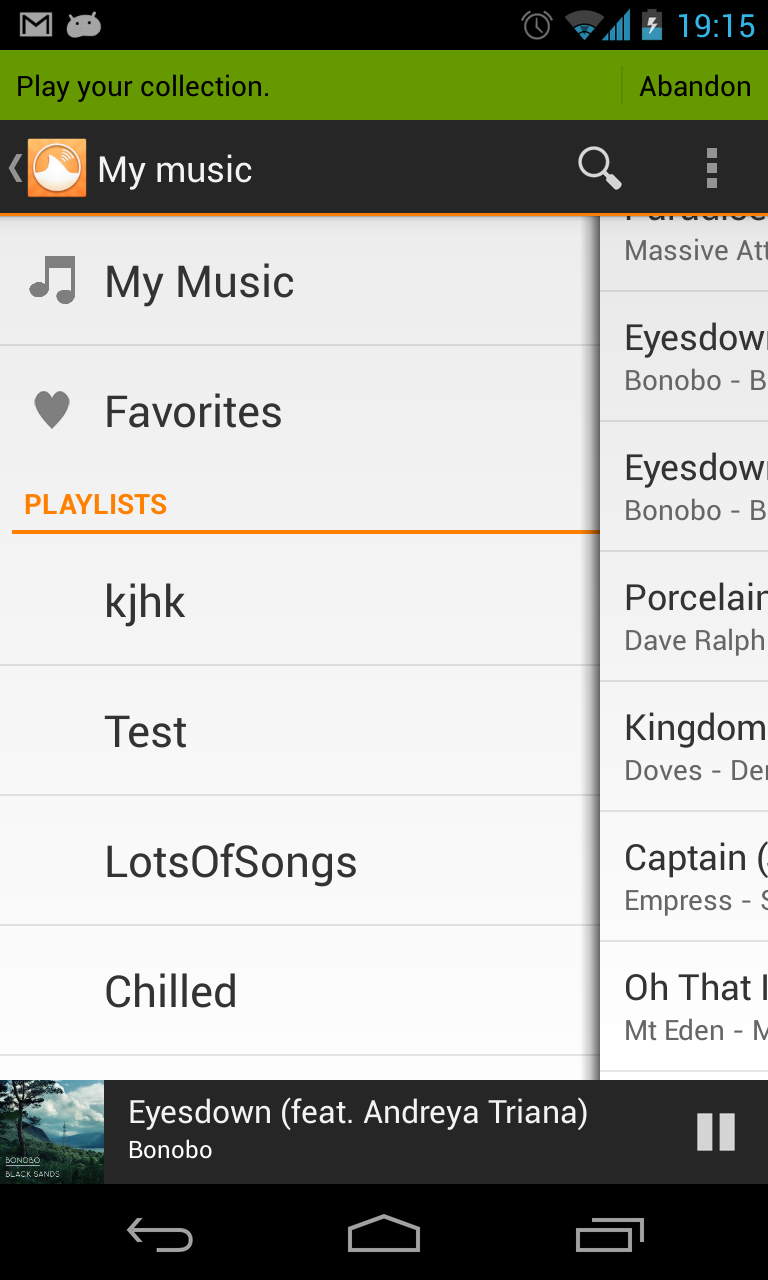
\includegraphics[width=0.5\textwidth]{images/updated-application}
  \caption{The testing running in the updated version of the application.}
  \label{fig:updated-application}
\end{figure}

\section{Ease of Testing}

This is the area where this library hopes to improve on ``think
aloud'' testing.

Again, the convenience this method provides depends on the application
being tested. Since it makes use of crowdsourcing, the quality of
results relies on having a number of people available to use it.
This might be trivial with an application which, for example, has
an existing beta program within an organisation. In this scenario
the testing library can be integrated into the version distributed
to the beta users and run when on the first use of the application,
or when a new feature to be tested is implemented.

If a something like this does not exist then there are other solutions
to this problem. One route would be Amazon Mechanical Turk (MTurk),
a well known web service where users perform short tasks for a small
payment - usually in the region of a few tens of cents (USD).
Although this involves money it still compares very favourably
with the amounts that are usually paid to testing participants, or
to services such as usertesting.com.

\section{Quality of the results}

To evaluate the effectiveness of the data gathered from the testing
process, a number of participants were given the test application
and told to complete all the tasks. The application used was the
same as the one used for designing and developing the library.
Since the application required some setup on the computer side,
which was not being tested, a laptop with the software installed
was provided to the participant. The tests were supervised to observe
how the participant coped with using the test system, but they were told
not to speak during the test or voice any opinion on the usability
of the app itself.

The tasks used are shown in Appendix~\ref{apdx:tasks} and the
result graphs generated by the web service in Appendix~\ref{apdx:graphs}. 
The success
rate and average total backtracks (the average backtracks a user
made during the entire task) are summarised in the table below.


\begin{tabular}{| c | c | c |}
\hline
Test Id & Success Rate & Average Total Backtracks \\
\hline
connect & 100\% & 1.2 \\
playlibrary & 33\% & 2.3\\
skipsong & 100\% & 0.3 \\
startshuffle & 100\% & 0.5 \\
search & 100\% & 2.8 \\
viewalbum & 83\% & 0.8 \\
addalbumtoplaylist & 0\% & 1.5 \\
\hline
\end{tabular}

\subsection{Low Completion Rates}

A number of things stand out from this summary. Two of the tasks had low completion
rates, one of which no participant managed successfully! This immediately indicates problems with
the user experience in these areas. Looking at the detailed graph of the ``addalbumtoplaylist''
task we see users taking a
number of different paths, but the majority of them end up on the album detail screen at some
point where many abandon the task. Looking at this screen ourselves reveals that although
there is a menu for more actions to perform on the album it omits the option to add
the entire album to a playlist. This option is present in the album menu on the artist
detail page, however no participant found it in this location. Disclaimer: This was
a bug in the version of the application used for the testing, which I had noticed just
prior to writing the tasks. This task was deliberately added out of curiosity, to evaluate
how the library would cope with a situation like this. The results are particularly pleasing,
and show how testing could have caught a bug like this quickly instead of the months it took
to notice otherwise.

The other task with a low completion rate is the ``playlibrary'' tasks. Here the results
highlight two things, which were also observed while watching the participants.
In the task introduction, participants are instructed to ``play their \emph{collection}'',
however in Grooveshark (and in the app) the concept of a user's collection is known as 
``My Library''. Because of this, some participants were left confused, with no obvious path
to take to get to their ``collection''. The navigation graph shows a fairly large number of
backtracks, with 50\%
of people abandoning the task without reaching the My Music screen,
even though it is the easiest screen to reach. Here we see the importance of wording 
tasks correctly - a regular
Grooveshark user would be looking for an area of the app called ``My Music'', so
calling it something else in the testing only serves to confuse participants.
Among participants who did reach the correct area of the app, however there is still
a high number of backtracks and users who abandoned the task indicating that they had trouble
finding the ``Play All'' button which is hidden in the application's overflow menu. Indeed, this mirrors
my findings after releasing the app, having received emails from users asking if this functionality
is available. Testing with this library before release could have highlighted this issue sooner.
The results showed that the issue might be wider than the email feedback indicated, and later
versions have an improved interface for this action.

\subsection{Other Usability Indicators}

Another task that stands out in the results is the ``search'' task, where the participants
were instructed to search for and play a specific song. Although the task has a 100\% completion
rate, the average number of backtracks are especially high, suggesting people
were unexpectedly struggling. The task should be relatively simple - all participants
began by searching for the name of the song, and the correct result appears near the top
in the list of song results. Instead, however, we see many people navigating to the artist
detail screen, and a high number of backtracks. Performing this search ourselves shows that
although the song is found, the app features artist and album results first, pushing the
song results off screen, and requiring the user to scroll to see them (Figure~\ref{fig:search-results}). It appears that people
have a tendency to click on the first item they see which has relevance to the result they
are searching for; in this instance the artist of the song, which appears near the top
of the screen. Here, the app lets them down, displaying a disorganised list of the artist's
albums in which the desired song is particularly hard to find. While all the participants did eventually
find the song here or by returning to the search screen, the experience could definitely be
improved. In a future version, I plan to show fewer album and artist results by default,
allowing the song results to be visible on the main search results screen. Another improvement
that could be made due to this feedback is showing the top songs by an artist on the artist
summary screen, and improving the album list layout.

\begin{figure}[h]
  \centering 
  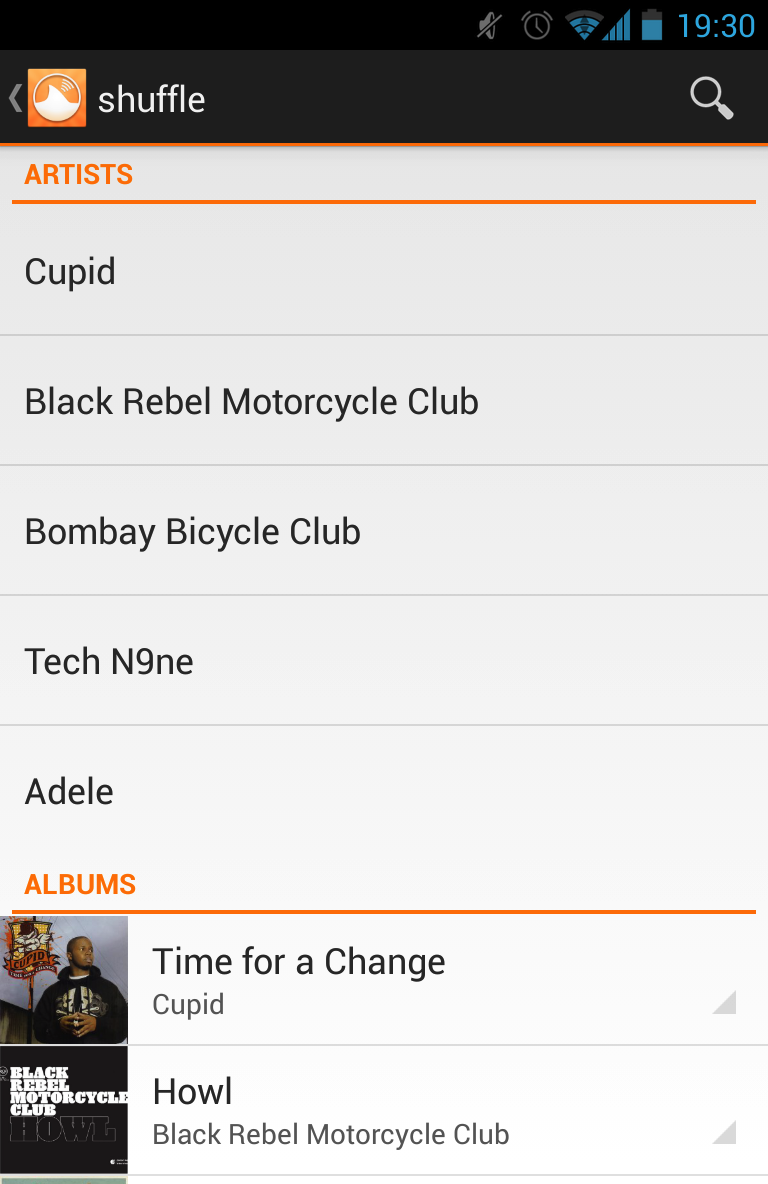
\includegraphics[width=0.5\textwidth]{images/search-results}
  \caption{The results screen that users saw when performing the search task.
           Notice that the artist (Bombay Bicycle Club) is shown near the top of the
           results, while the actual song is pushed off screen below the album
           results.}
  \label{fig:search-results}
\end{figure}

\subsection{Tests Usability}

After gathering feedback about the testing process from participants,
some of them expressed they wished they
could revisit the instruction page after starting a task, to make sure they
had read the task correctly. One or two participants occasionally didn't
read the task description fully before starting, which explains the multiple
routes taken in the ``viewalbum'' task. Although most participants completed the
task, it didn't necessarily test the usability of the use case the task was designed
to test. It is, at least, quite obvious what happened from the navigation graph,
with some users immediately searching for the song despite the instructions.

\section{Future Work}

\subsection{Library Enhancements}

Depending on the task and the application being tested, the user 
evaluation highlighted a problem with the library which arises
due to the ability to abandon tasks, and when a subsequent task
depends on state set in a previous, abandoned task. The most 
obvious example in the application here is the initial pairing
and connecting, which none of the subsequent tasks can be done
without. During evaluation the ability to abandon this first task
was disabled to combat this, and luckily no participant was unable
to complete the challenge.

The same problem, however, appeared later during the third task, when
the participant is told to skip to the next song in the play queue.
If the previous task had not been successfully completed there was a
chance that either nothing would be playing, or the play queue would
only be holding a single track making the task confusing and nonsensical
to the participant. Even if they then add songs to the queue, it affects
the navigation path generated for the task.

In a future revision of the library, the obvious way to solve the above issue
would be to allow the app developer to provide logic to run in the event
a task is abandoned. In this example, the library could look for a
particular class with the static method \verb/playlibrary_Abandoned()/
using Java reflection and invoke it. The method would simply insert
songs into the play queue in preparation for the subsequent tasks.

Other enhancements could be made in the area of task delivery. Perhaps
the option of playing a recording of the developer reading the task
description, or even a video, would make tasks descriptions less likely
to be misinterpreted.

\subsection{Results and Data}

This project concentrated on the capture of navigation data, and a single
way of presenting the results. Once the framework is implemented into the
application many other forms of data could be captured during the testing
process with the aim of providing more detail about user behaviour and
issues.

There is much scope to improve the results display with greater interactivity,
such as:

\begin{itemize}
  \item Filtering the view to show only completed or abandoned navigations.
  \item Highlighting all paths which go through a particular navigation point.
  \item Highlighting longer than usual navigation chains, and ones which only end in failure.
  \item Showing more information about backtracks, such as where the users
        navigate before backtracking.
\end{itemize}


One example of a greater extension to the project might be to provide heatmaps
of user interaction on each screen. Since the library already has the
capability to inject views into the current layout, it should be possible
to overlay a transparent view that serves to capture touch information
whenever the participant uses the screen. Similar approaches are already
used in user testing on the web and desktop, and the same system could
be used with both traditional in-person testing and crowdsourced testing.


\subsection{Combination With Other Tests}

The library could be combined with an A/B testing library, and participants
given slight variations of parts of the interface. Using this combination, 
when issues are detected then the performance of different interface fixes
could be tested, comparing the performance of each to each other and the original.